\documentclass[11pt]{article}
\usepackage[utf8]{inputenc}
\usepackage[T1]{fontenc}
\usepackage[spanish,provide=*]{babel}
\usepackage[a4paper,margin=2.4cm]{geometry}
\usepackage{amsmath,booktabs,graphicx,url,tikz}
\title{Test 5: malla, error de campo y contorno}
\author{Almendra Olivares Bravo}
\date{}
\begin{document}
\maketitle
\section{Problema y referencia}
Se estudia una barra axial elástica con $L=2000$ mm, $E=200000$ N/mm$^2$, $A=1000$ mm$^2$, $P=20000$ N y $q=10$ N/mm. Las cargas actúan hacia $+x$; $E$ y $A$ son constantes. Se busca determinar si el acuerdo nodal basta para aceptar el campo MEF y distinguir refinamiento de malla de cambio de contorno.
\begin{center}
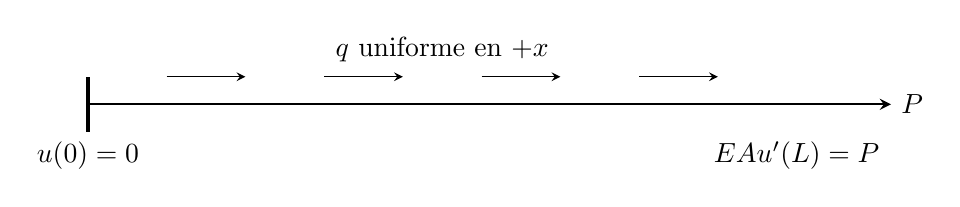
\begin{tikzpicture}[>=stealth]
\draw[very thick] (0,0)--(0,0.7);
\draw[thick] (0,0.35)--(9,0.35);
\foreach \x in {1,3,5,7}{\draw[->] (\x,0.7)--(\x+1,0.7);}
\draw[->,thick] (9,0.35)--(10.2,0.35) node[right] {$P$};
\node at (4.5,1.05) {$q$ uniforme en $+x$};
\node[below] at (0,0) {$u(0)=0$};
\node[below] at (9,0) {$EAu'(L)=P$};
\end{tikzpicture}
\end{center}
Integrando $-(EAu')'=q$ se obtiene $EAu'=-qx+C_1$ y $EAu=-qx^2/2+C_1x+C_2$. Las condiciones de borde dan $C_1=P+qL$ y $C_2=0$:
\[
u_{\rm ref}(x)=\frac{(P+qL)x-qx^2/2}{EA},\qquad u_{\rm ref}(L)=0{,}300\ \mathrm{mm}.
\]
\section{Método y resultados}
Se conserva el solver suministrado: elementos lineales uniformes, cargas consistentes y solución de $K_{ff}u_f=f_f$ mediante \texttt{numpy.linalg.solve} \cite{numpy}. Se implementan la referencia y el error en los puntos medios, con $h=L/n$:
\[
x_{m,e}=\frac{x_i+x_{i+1}}2,\quad u_h(x_{m,e})=\frac{u_i+u_{i+1}}2,\quad e_m=\max_e|u_h(x_{m,e})-u_{\rm ref}(x_{m,e})|.
\]
\begin{center}
\begin{tabular}{rrrrrr}
\toprule
$n$ & $h$ [mm] & $u(L)$ [mm] & $R_0$ [N] & balance [N] & $e_m$ [mm]\\
\midrule
2 & 1000 & 0,300 & $-40000$ & 0 & 0,006250000\\
4 & 500 & 0,300 & $-40000$ & $2{,}18\,10^{-11}$ & 0,001562500\\
8 & 250 & 0,300 & $-40000$ & $-3{,}64\,10^{-11}$ & 0,000390625\\
\bottomrule
\end{tabular}
\end{center}
Aquí $e_m=|q|h^2/(8EA)$: al duplicar $n$, el error se divide por cuatro. El acuerdo nodal es propio de este caso de $EA$ constante y carga uniforme; la interpolación lineal no reproduce la parábola entre nodos.
\newpage
\section{Verificación y cambio de contorno}
Con $K$ y $f$ originales se calcula $r=Ku-f$: en los grados libres $r_f\approx0$ y en los restringidos $r_c=R_c$. En los cuatro casos, $\max|r_f|\leq5{,}82\,10^{-11}$ N. El balance relativo $|\sum R+P+qL|/|P+qL|$ es como máximo $9{,}09\,10^{-16}<10^{-8}$. Las dos pruebas base pasan; esto verifica el cálculo, no constituye validación experimental.

Con 8 elementos se agrega $u(L)=0$ manteniendo las cargas. La nueva referencia es $u_a(x)=qx(L-x)/(2EA)$, con $R_0=-10000$ N y $R_L=-30000$ N. La fuerza $P$ aplicada sobre el apoyo derecho se compensa en su reacción. Así, $-10000-30000+20000+20000=0$, aunque se resolvió otro problema. En el centro, $u$ pasa de $0{,}175$ a $0{,}025$ mm; en el extremo derecho, de $0{,}300$ a cero.
\begin{figure}[h]
\centering
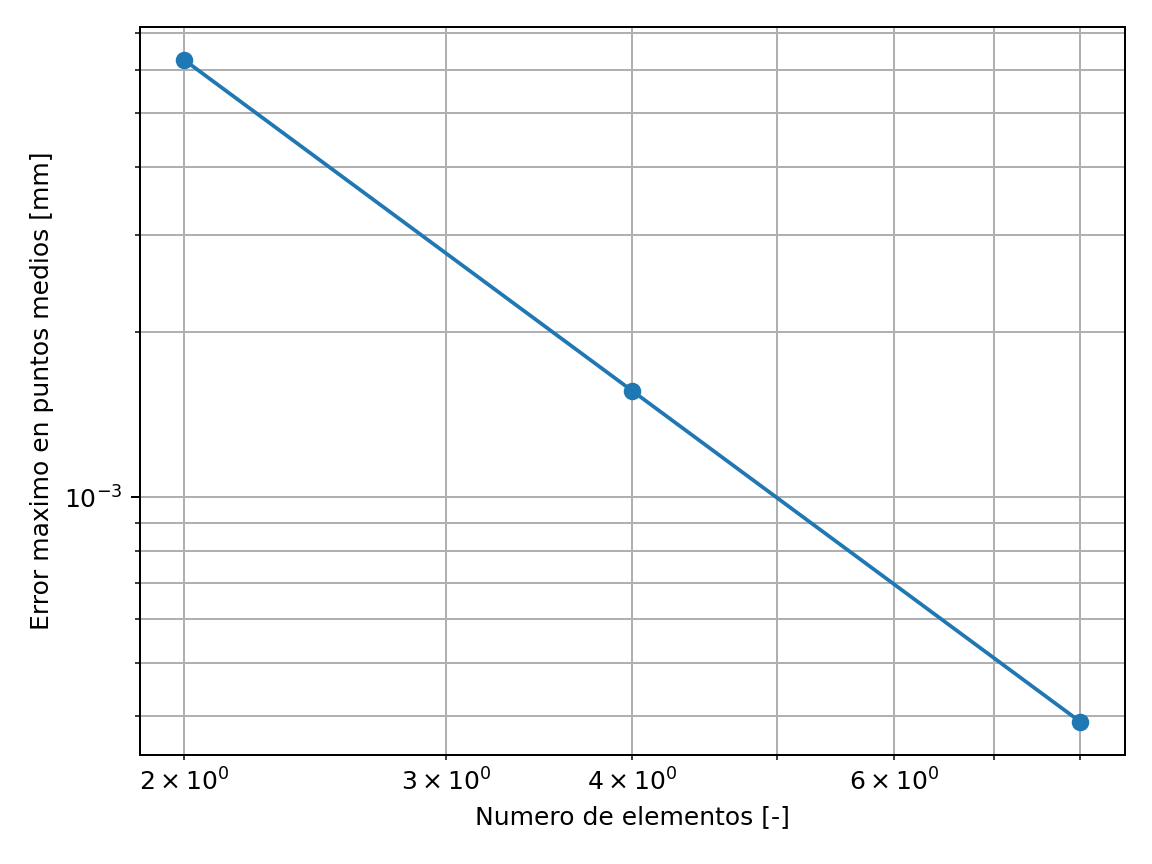
\includegraphics[width=0.48\linewidth]{../salidas/convergencia.png}\hfill
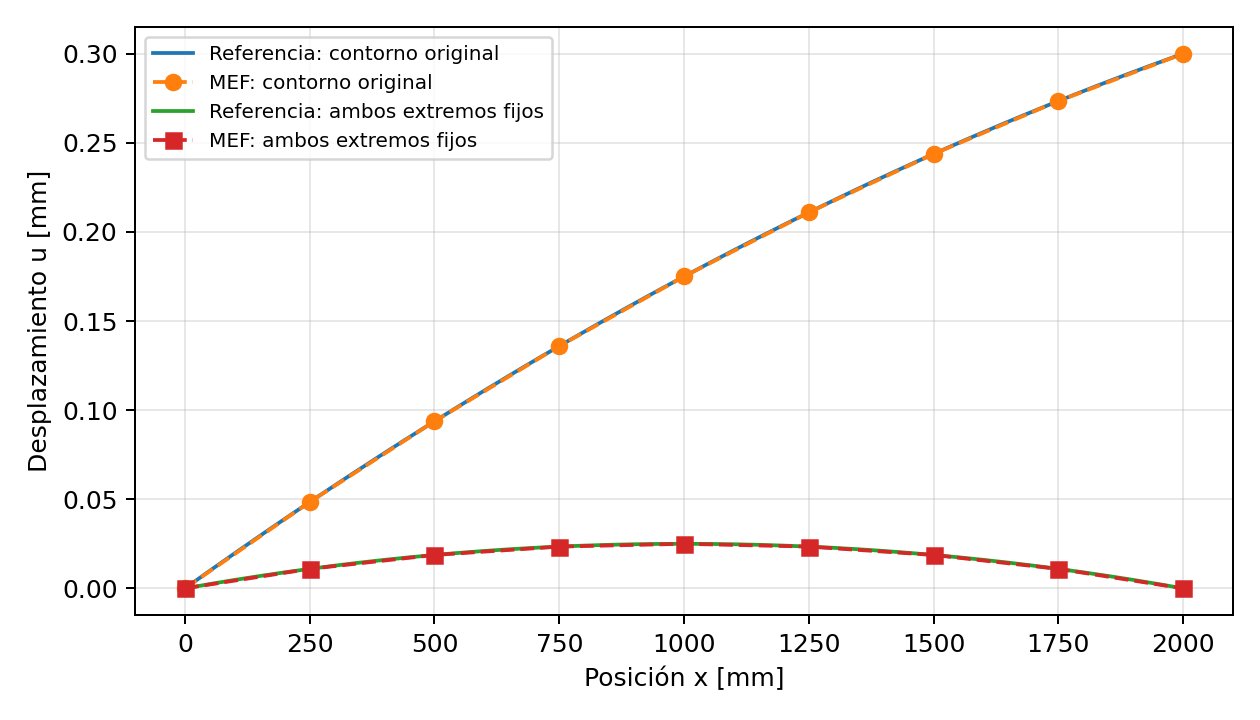
\includegraphics[width=0.49\linewidth]{../salidas/comparacion_contornos.png}
\caption{Error al refinar (izquierda) y desplazamientos con 8 elementos para ambos contornos (derecha).}
\end{figure}
\section{Conclusión}
El acuerdo nodal no basta para aceptar el campo aproximado: los elementos lineales unen valores exactos, pero no reproducen la curvatura entre nodos. El error disminuye como $h^2$, sin cambiar $u(L)$ en este caso. Agregar el apoyo derecho modifica desplazamientos y reacciones porque cambia el problema de borde. Ambos modelos satisfacen equilibrio, de modo que un residuo pequeño no asegura que las restricciones representen el problema original. La credibilidad exige revisar conjuntamente referencia, error de campo y condiciones de borde.
\section*{Trazabilidad y uso de IA}
Resultados de Colab en \texttt{salidas/resultados.csv}, \texttt{verificacion.csv} y \texttt{comparacion\_contornos.csv}; decisiones en \texttt{BITACORA.md}. Las expectativas fueron guiadas después de conocer resultados de referencia. Se utilizó ChatGPT para derivación, código de análisis, interpretación y preparación del informe; se contrastaron resultados con fórmulas analíticas, residuos y pruebas. Se conservó el solver base. Detalle en \texttt{USO\_IA.md}.
\bibliographystyle{plain}
\bibliography{referencias}
\end{document}
